%%%%%%%%%%%%%%%%%%%%%%%%%%%%%%%%%%%%%%%%%%%%%%%%%%%%%%%%%%%%%%%%%%%%%%%
\chapter{Basic Bond Graph Elements}
\label{ch:elements}
%%%%%%%%%%%%%%%%%%%%%%%%%%%%%%%%%%%%%%%%%%%%%%%%%%%%%%%%%%%%%%%%%%%%%%%

A remarkably small set of ideal elements suffices to model the dynamics of systems across all energy domains. There are \textbf{nine} fundamental bond graph elements: three 1-port passive elements (R, C, I), two source elements (Se, Sf), two 2-port elements (TF, GY), and two junction elements (0-junction, 1-junction). Every physical system model is assembled from these building blocks. 

Real devices can be considered as subsystems from the point of view of power exchanges and external port variables. These basic multiport elements are idealized mathematical models,or conceptual "entities",used to model specific physical effects within a device. The bond graph notation often allows one to visualize aspects of the system structure more easily than with state equations or graphical notations designed strictly for a single energy domain.

\section{The 1-port resistor \textit{R}: energy dissipation}

A resistor is a 1-port in which effort and flow are related by a \textbf{static constitutive law} $e = \mathcal{R}(f)$ (or equivalently $f = \mathcal{R}^{-1}(e)$). 

No energy is stored: whatever power enters the port is dissipated instantly (converted to heat in the thermal domain, which is usually neglected in the model). In the $e$--$f$ plane, a passive resistor's constitutive curve lies in the first and third quadrants, ensuring $ef \geq 0$ (power always flows in). Power flows into the port when the product of $e$ and $f$ is positive according to the assigned sign convention. Because energy seems to disappear from the electrical, mechanical, or hydraulic domains, it is in reality transferred into the thermal domain, whose presence is typically neglected in these basic dynamic models.

\begin{figure} [H]
\centering
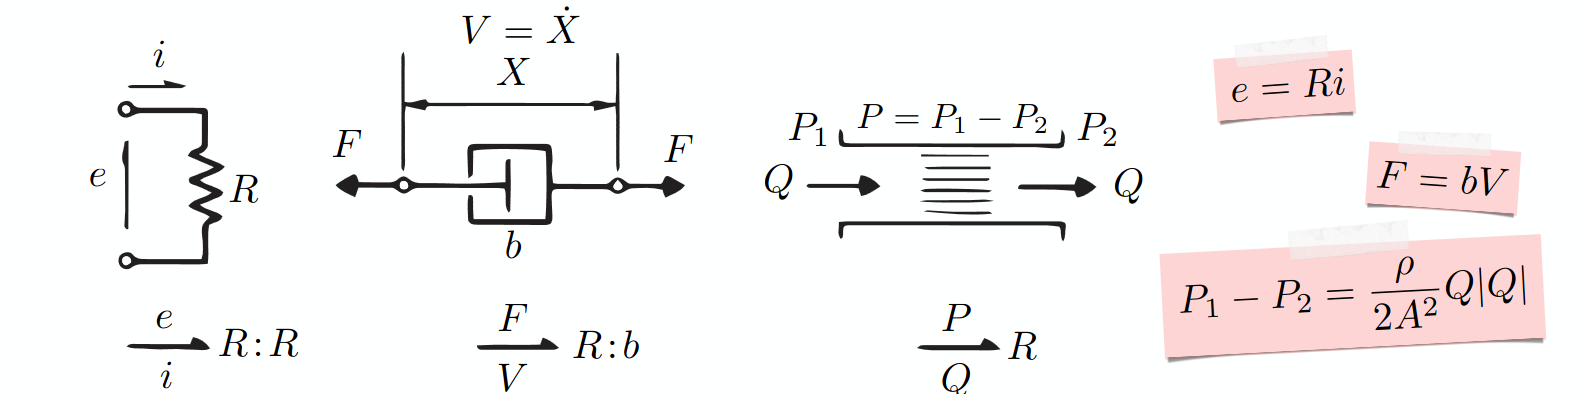
\includegraphics[scale=0.25]{figs/chapter2/2_1.png}
\caption{Different types of Resistive 1-port elements.}
\end{figure}

Physical realisations: electrical resistance $e=Ri$; viscous damper $F=bV$; fluid resistance $\Delta P = R_f Q$ (linear); orifice flow $\Delta P = k Q|Q|$ (nonlinear). 

In the bond graph:
\begin{center}
\begin{tikzpicture}[>=Stealth,every node/.style={font=\small}]
  \draw[thick,-stealth] (0,0) -- (1.2,0);
\node[draw,fill=gray!12,minimum width=1.0cm,minimum height=0.7cm,font=\small\bfseries]
    at (1.9,0) {R};
  \node at (-0.3,0.25) {$e$}; \node at (-0.3,-0.25) {$f$};
\node[font=\footnotesize,gray] at (5,0) {constitutive: $e=\mathcal{R}(f)$};
\end{tikzpicture}
\end{center}
The half-arrow points toward R (positive power convention). \textbf{For a linear element: appending \texttt{R:R} (or \texttt{R:b} for a damper) names the parameter}.


\begin{insightbox}[Causality of R]
The causality of a resistor is not fixed: it can be either effort-in or flow-in. This is because the constitutive relation is static, so if you impose one variable, the other is immediately determined without any integration or differentiation.
\end{insightbox}

\section{The 1-port capacitor \textit{C}: potential energy storage}

A capacitor (or compliance) stores \textbf{potential energy} via a static relationship between effort and displacement:
\begin{equation}
  e = \mathcal{C}^{-1}(q), \qquad q = \int f\,dt.
\end{equation}
In the linear case, $e = q/C$. The linear compliance $C$ is defined as the inverse of the slope of the $e$ versus $q$ constitutive curve.

Stored energy:
\begin{equation}
  E(q) = \int_{q_0}^q e(\bar{q})\,d\bar{q} \quad\longrightarrow\quad E = \frac{q^2}{2C} \text{ (linear)}.
\end{equation}

Usually $E_0$ is set to zero by offsetting the energy reference point.

Since the capacitor stores energy without loss, the power flow into the port can reverse, meaning power flows back out into the system. During this process, energy is strictly conserved.

\begin{figure} [H]
  \centering
  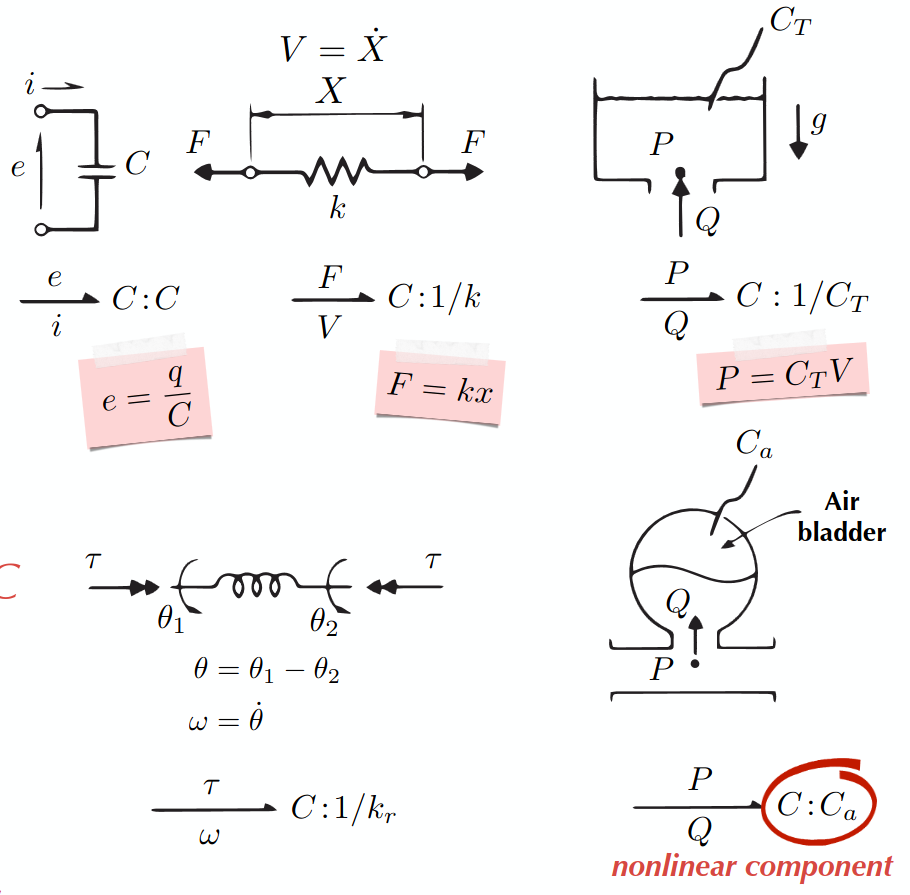
\includegraphics[scale=0.25]{figs/chapter2/2_2.png}
  \caption{Different types of Capacitive 1-port elements.}  
\end{figure}

Physical realisations: electrical capacitor $e = q/C$; spring $F = kx$ (so $C = 1/k$); hydraulic accumulator $P = V/C_a$; torsional spring $\tau = k_r\theta$.

\begin{insightbox}[Preferred causality of C]
A capacitor can either be in \textbf{integral causality} and in \textbf{derivative causality}.

$$
  e = \mathcal{C}^{-1}\biggl(\int f\,dt\biggr), \qquad f = \frac{d}{dt} \mathcal{C}(e).
$$

The natural causality for a capacitor is \textbf{flow-in, effort-out}: flow is integrated to give displacement, from which effort is computed. This is called \emph{integral causality}. If the bond graph forces effort-in on C (derivative causality), the element does not contribute an independent state variable, which has implications for the system's order.

Intuitively, from a simulation perspective, you impose the flow (e.g., current or velocity) which the element integrates into displacement (charge or position), and this displacement yields the effort (voltage or force) as an output.
\end{insightbox}

\section{The 1-port inertia \textit{I}: kinetic energy storage}

An inertia (inductor) stores \textbf{kinetic energy} via a static relationship between flow and momentum:
\begin{equation}
  f = \mathcal{I}^{-1}(p), \qquad p = \int e\,dt.
\end{equation}
In the linear case, $f = p/I$. Here, the linear inertia $I$ is defined as the inverse of the slope of the $f$ versus $p$ curve.

Stored energy:
\begin{equation}
  E(p) = \int_{p_0}^p f(\bar{p})\,d\bar{p} \quad\longrightarrow\quad E = \frac{p^2}{2I} \text{ (linear)}.
\end{equation}

Similarly to the capacitor, the $E_0$ reference point is typically set to zero.

\begin{figure} [H]
  \centering
  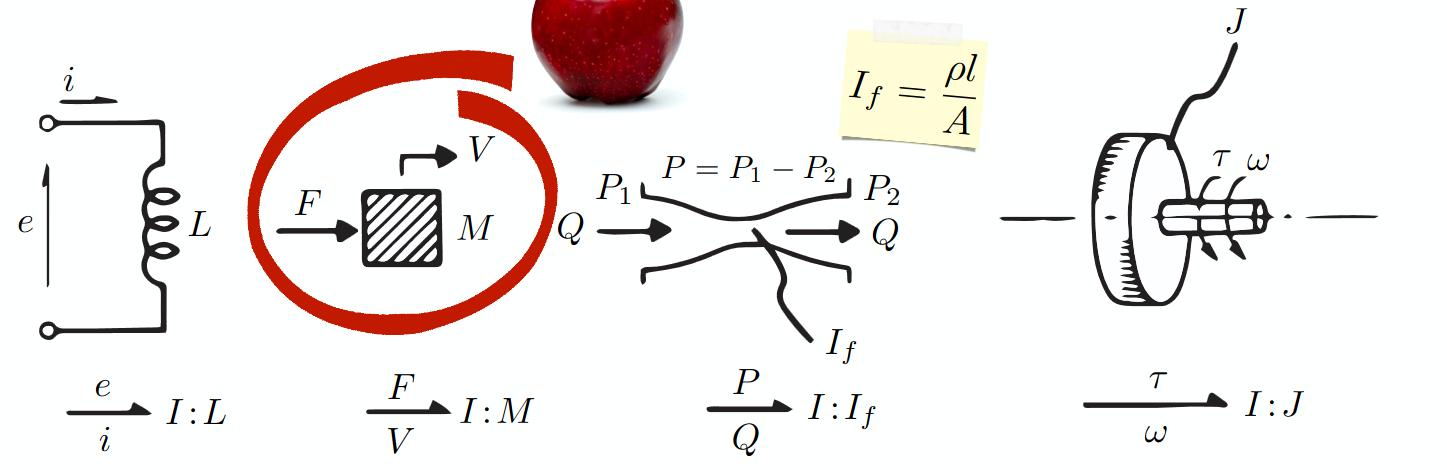
\includegraphics[scale=0.25]{figs/chapter2/2_3.png}
  \caption{Different types of Inertial 1-port elements.}
\end{figure}

Physical realisations: point mass $F = ma \Rightarrow V = P/m$ (so $I = m$); rotating body $\tau = J\dot{\omega} \Rightarrow \omega = p_\tau/J$; fluid inertance $\Delta P = I_f \dot{Q}$.

\begin{insightbox}[Preferred causality of I]
An inertia integrates force to give momentum, which means that it accumulates the effect of effort over time. The formula is $v = p/I$, so the flow (velocity) is derived from the momentum, which is $p = \int e\,dt$. If it was otherwise, and you imposed the flow (velocity), it would mean that imposing an abrupt change in velocity would require an infinite force, which is not physically realizable. 

\begin{equation}
  f = \mathcal{I}^{-1}\biggl(\int e\,dt\biggr), \qquad e = \frac{d}{dt} \mathcal{I}(f).
\end{equation}

The natural causality for an inertia is \textbf{effort-in, flow-out}: effort is integrated to give momentum, from which flow is computed. Again, this is integral causality. Newton's second law is a direct statement of this: force (effort) integrates to momentum, from which velocity (flow) is recovered. 

As with the capacitor, imposing flow on an inertia leads to derivative causality because the imposed flow must be differentiated to find the required effort, thus reducing the number of independent state variables (you lose position, hence memory).
\end{insightbox}

The tetrahedron of state variables  summarises the four types and their relationships: $\dot{p}=e$, $\dot{q}=f$, with C linking $e$--$q$ and I linking $f$--$p$.

\begin{figure} [H]
  \centering
  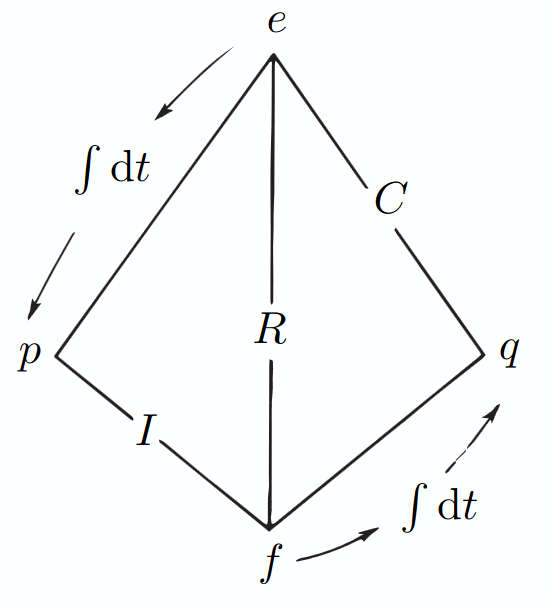
\includegraphics[scale=0.25]{figs/chapter2/2_4.png}
  \caption{Tetrahedron of state variables.}
\end{figure}

\section{Source elements \textit{Se} and \textit{Sf}}

An \textbf{effort source} $Se$ maintains a specified effort $e(t)$ at its port, regardless of the flow (infinite power if needed, the idealisation of a stiff voltage/force/pressure supply). A \textbf{flow source} $Sf$ dually maintains a specified flow. 

\textbf{Their causality is fixed}: $Se$ always imposes effort (causal stroke away from $Se$); $Sf$ always imposes flow.

\begin{figure} [H]
  \centering
  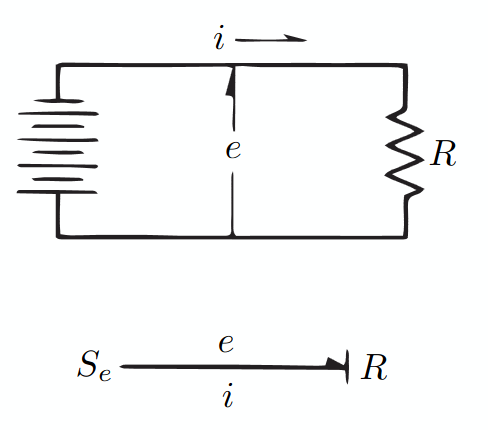
\includegraphics[scale=0.25]{figs/chapter2/2_5.png}
  \caption{Example of source elemets. Voltage generator and resistor in series, with $Se$ imposing voltage and $R$ determining current.}
\end{figure}

In reality, components always find a compromise. For instance, when you set the voltage of a real battery, the act of drawing current inherently lowers the voltage itself. Because ideal sources do not model this compromise in one go, a real-world component like a battery must be modeled using an ideal voltage source ($Se$) in series with a resistance ($R$) to accurately simulate the voltage drop under load.

When the source value is itself a function of a signal from another part of the graph, it becomes a \textbf{modulated source} MSe or MSf. This is how controlled actuators, variable-flow pumps, and vibration shakers are represented.

\begin{figure} [H]
  \centering
  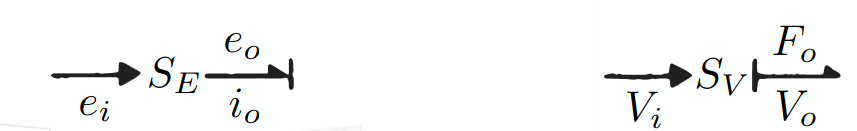
\includegraphics[scale=0.25]{figs/chapter2/2_6.png}
  \caption{Modulated source of effort (MSe) and modulated source of flow (MSf).}
\end{figure}

\section{The transformer \textit{TF}: effort--effort, flow--flow exchange}

A transformer is a \textbf{power-conserving 2-port}: $e_1 f_1 = e_2 f_2$ at all times. Its constitutive relations scale effort and flow by a constant (or time-varying) modulus $m$:
\begin{equation}
  \begin{cases}
    e_1 = m \, e_2 \\
    m \, f_1 = f_2
  \end{cases}
\end{equation}
Effort is scaled up by $m$, flow is scaled down by $m$ (or vice versa).

\begin{figure}[H]
  \centering
  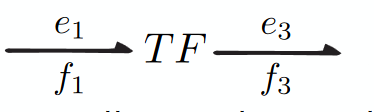
\includegraphics[scale=0.25]{figs/chapter2/2_7.png}
  \caption{Bond graph symbol for the transformer element.}
\end{figure}


Physical examples: electrical transformer ($m = N_1/N_2$, turns ratio); lever ($m = b/a$, arm ratio); hydraulic piston ($F = AP$, $AV = Q$, so $m = A$); gear pair ($m = r_1/r_2$); rack and pinion.

\begin{figure}[H]
  \centering
  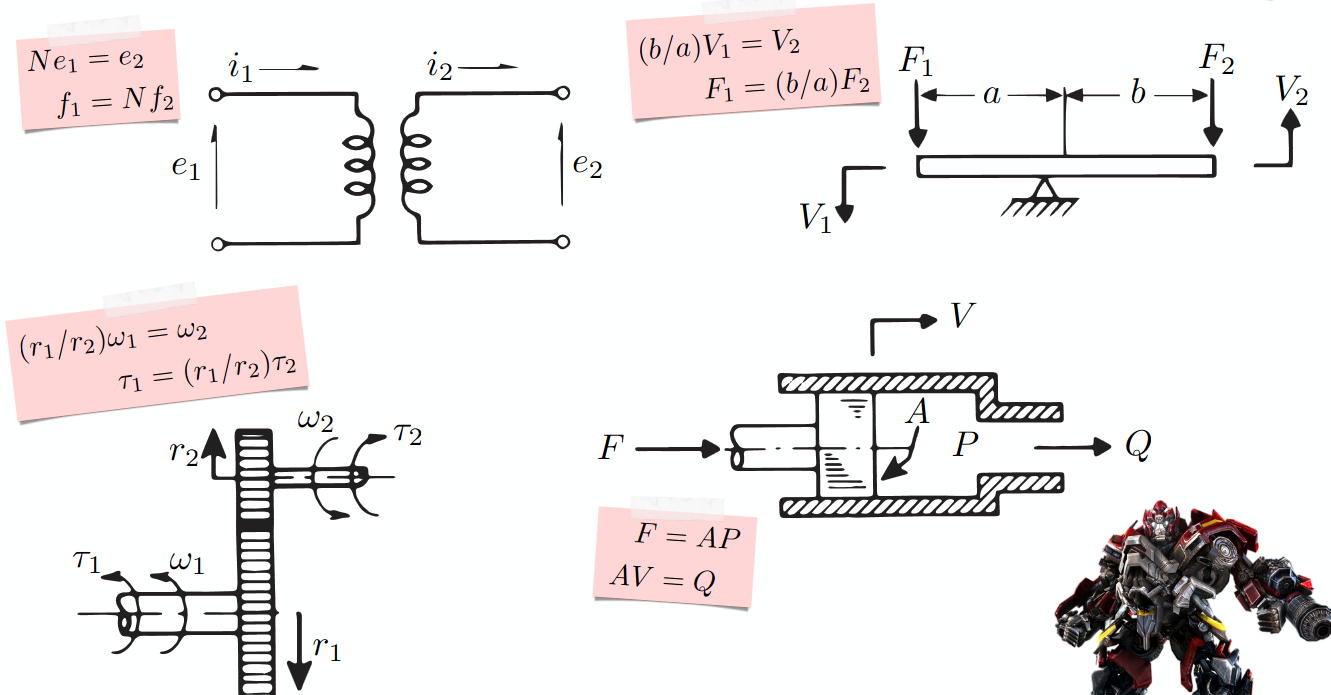
\includegraphics[scale=0.25]{figs/chapter2/2_8.png}
  \caption{Physical examples of transformer elements.}
\end{figure}


\begin{insightbox}[TF causality]
Two causal forms are valid for TF: either effort-in on port 1 (and effort-out on port 2), or effort-in on port 2. The causal stroke must appear on exactly one of the two ports. 

\end{insightbox}

If the geometry changes (e.g.\ a linkage), $m$ becomes time-dependent, the element becomes a \textbf{modulated transformer} MTF. 
\begin{figure} [H]
  \centering
  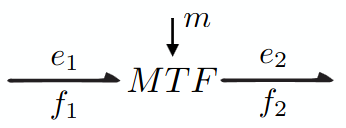
\includegraphics[scale=0.25]{figs/chapter2/2_14.png}
  \caption{Modulated transformer (MTF).}
\end{figure}

In robotics, the Jacobian matrix plays the role of the MTF modulus. The Jacobian expresses the relationship between end-effector and joint velocities ($v = J(\theta)\dot{\theta}$). Assuming power conservation, it naturally also relates the end-effector applied force to the joint torques ($\tau = J^T(\theta)F$).

\section{The gyrator \textit{GY}: effort--flow exchange}

A gyrator is also power-conserving, but it exchanges the roles of effort and flow:
\begin{equation}
  e_1 = r\,f_2, \qquad r\,f_1 = e_2.
\end{equation}

\begin{figure} [H]
  \centering
  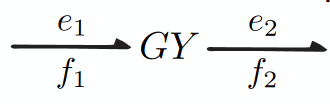
\includegraphics[scale=0.25]{figs/chapter2/2_9.png}
  \caption{Bond graph symbol for the gyrator element.}
\end{figure}

This is fundamentally different from TF: while a transformer maps effort to effort and flow to flow through a constant, the gyrator maps a flow to an effort and vice versa through a constant. 

\begin{figure}[H]
  \centering
  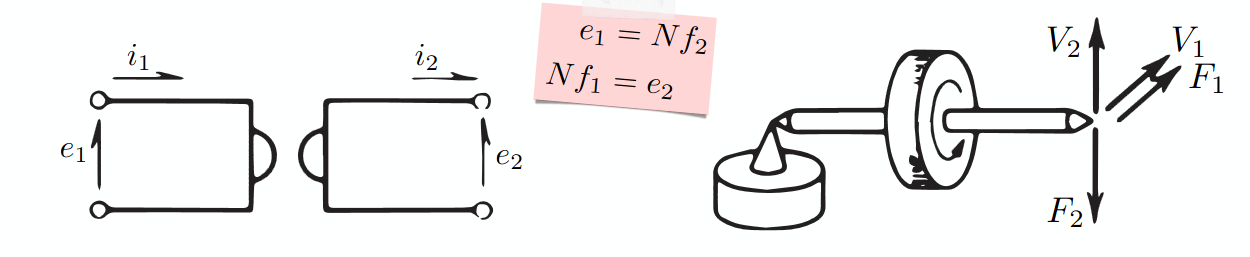
\includegraphics[scale=0.25]{figs/chapter2/2_10.png}
  \caption{Example of gyrator element.}
\end{figure}

\begin{figure}[H]
  \centering
  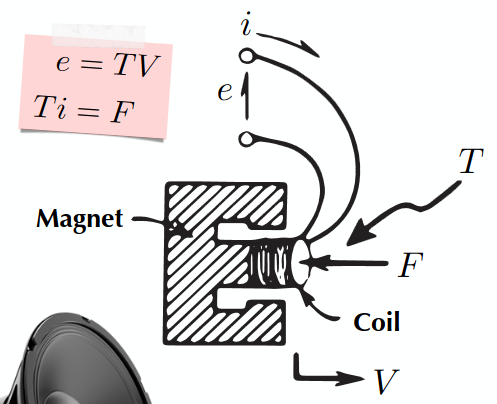
\includegraphics[scale=0.25]{figs/chapter2/2_11.png}
  \caption{More example of gyrator element.}
\end{figure}

Physical examples: DC motor (back-EMF $e_a = T\omega$, torque $Ti_a = \tau$, so $r = T$); gyroscope (a force in one direction induces an angular velocity in the perpendicular direction).

\begin{insightbox}[Gyrator is more fundamental than transformer]
The gyrator can sometimes seem like a mysterious element, but it is actually more fundamental than a transformer. Two cascaded gyrators produce a transformer. 

\begin{figure} [H]
  \centering
  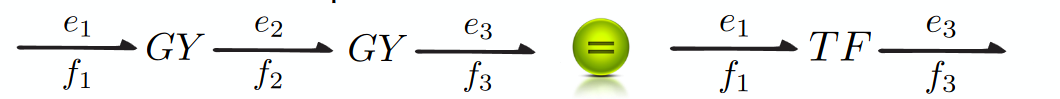
\includegraphics[scale=0.25]{figs/chapter2/2_12.png}
  \caption{Gyrator as a fundamental element.}
\end{figure}

More profoundly, a gyrator essentially interchanges the roles of effort and flow, so it maps C-elements into I-elements: a capacitor seen through a gyrator behaves as an inertia. This means one does not fundamentally need two types of energy-storage elements, the gyrator generates one from the other. Historically, ignoring gyrators and forcing gyroscopic systems into transformer notation led to incorrect models.

\begin{figure} [H]
  \centering
  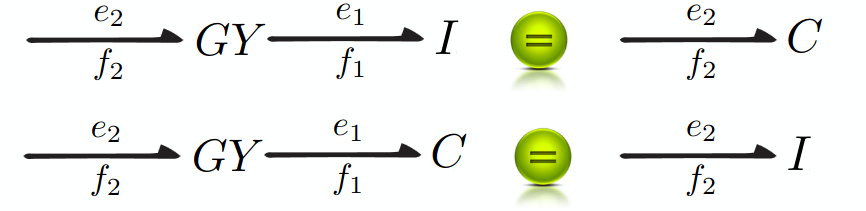
\includegraphics[scale=0.25]{figs/chapter2/2_13.png}
  \caption{Gyrator mapping C to I and vice versa.}
\end{figure}

\end{insightbox}


When the gyration ratio $r$ depends on a signal (e.g.\ motor torque constant varying with field current), the element becomes a modulated gyrator \textbf{MGY}.

\begin{figure} [H]
  \centering
  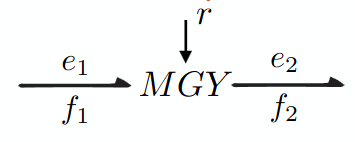
\includegraphics[scale=0.3]{figs/chapter2/2_15.png}
  \caption{Modulated gyrator (MGY).}
\end{figure}

\section{Junction elements: 0-junction and 1-junction}

Junctions are \textbf{power-conserving} multi-port elements that distribute power among connected elements. They enforce algebraic constraints on efforts and flows. Fundamentally, zero and one junctions are simply mathematical \textbf{conditions} applied to the system (such as force balance, flow conservation, or parallel branches sharing the same voltage).

\subsection{The 0-junction: common effort}

At a 0-junction all connected bonds share the \textbf{same effort}, and the flows sum algebraically to zero (with signs set by the half-arrow directions):
\begin{equation}
  e_1 = e_2 = e_3 = \cdots, \qquad \sum_k \pm f_k = 0.
\end{equation}

\begin{figure}[H]
  \centering
  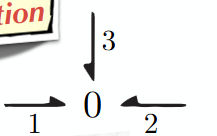
\includegraphics[scale=0.4]{figs/chapter2/2_16.png}
  \caption{Bond graph symbol for the 0-junction element.}
\end{figure}

Electrical analogue: a \textbf{node} (Kirchhoff's current law, same voltage). Mechanical analogue: a point where a single force acts on several elements with velocities that sum to zero (geometric compatibility, spring and damper in parallel). Here, we are imposing a relation between relative velocities. Hydraulic analogue: a junction of pipes (conservation of volume flow).

\subsection{The 1-junction: common flow}

At a 1-junction all connected bonds share the \textbf{same flow}, and the efforts sum algebraically to zero:
\begin{equation}
  f_1 = f_2 = f_3 = \cdots, \qquad \sum_k \pm e_k = 0.
\end{equation}

\begin{figure} [H]
  \centering
  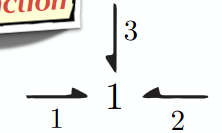
\includegraphics[scale=0.4]{figs/chapter2/2_17.png}
  \caption{Bond graph symbol for the 1-junction element.}
\end{figure}

Electrical analogue: a \textbf{loop} (Kirchhoff's voltage law, same current). Mechanical analogue: Newton's law for a mass, all forces acting on an inertia sharing a single velocity must balance. It encodes the action-reaction principle and effectively acts as a rigid connection among the mechanical elements. Hydraulic analogue: pressure drops around a single-flow circuit sum to zero.



\begin{warningbox}[Sign conventions at junctions]
The algebraic sum at a junction depends on the \emph{direction of the half-arrows}. One convention: at a 0-junction, the half-arrow of the ``driving'' bond points \emph{toward} the junction, and all others point away, then the sum of all $f_k$ equals the driving flow
\end{warningbox}

\subsection{Bond graph identities and simplification}

A 0-junction with only two bonds connecting to it reduces to direct connection (same effort, same flow). A 1-junction with only two bonds similarly reduces. These \textbf{bond graph identities} allow systematic simplification of an initial, verbose bond graph into a compact one. They are used heavily when eliminating zero-power bonds (e.g.\ after connecting to ground in a mechanical model) and when simplifying ``reducible loops'' that appear when spring and damper share the same relative velocity.

For \textbf{generalizing n-port components} there exist specific rules. 

\begin{figure} [H]
  \centering
  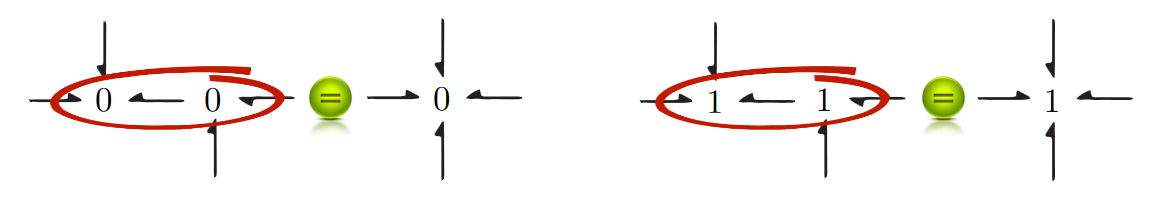
\includegraphics[scale=0.25]{figs/chapter2/2_18.png}
  \caption{Rules for simplifying n-port elements}
\end{figure}

\section{Causality summary for basic elements}

For effort and flow sources, causality is trivial and fixed. For basic 2-ports (TF, GY), there are two possible causal assignments; as soon as one variable is assigned as an input, the other is constrained by the constitutive relation. Similar logic naturally extends to 3-ports (junctions).


\begin{center}
\begin{tabular}{llll}
  \toprule
  \textbf{Element} & \textbf{Preferred causality} & \textbf{Alternative} & \textbf{Notes}\\
  \midrule
  Se & effort out (fixed) & - & always imposes $e$\\
  Sf & flow out (fixed) & - & always imposes $f$\\
  R  & either & either & indifferent (usually)\\
  C  & flow in (integral) & effort in (derivative) & derivative $\Rightarrow$ dependent state\\
  I  & effort in (integral) & flow in (derivative) & derivative $\Rightarrow$ dependent state\\
  TF & one of two forms & - & must be one in, one out\\
 
  GY & both in \emph{or} both out & - & two valid forms\\
  0-jct & one effort in, rest out & - & uniquely determined\\
  1-jct & one flow in, rest out & - & uniquely determined\\
  \bottomrule
\end{tabular}
\end{center}


Causality and bond graphs are very important. Indeed it's possible to predict many important features of the system
even before the constituitve laws for all the elements have been specified. 

It's possible to predict the number of state variables and it's useful for writing state equations. 

\vspace{0.5cm}


Once the causal stroke is added, it's possible to transform the bond graph into a block diagram.
They are more complex since a single bond represent two signal flows.